\chapter{Komponenten}
Nachdem im vorherigen Kapitel der grundlegende Aufbau des Funktionsgenerators erklärt wurde, sollen nun die einzelnen Komponenten aus denen der Funktionsgenerator aufgebaut ist genauer erläutert werden.
Vorab muss noch erwähnt werden, dass jede Komponente über ein \bit{CLK} und ein \lowactive{CE} Signal verfügen.
\lowactive{CE} ist der Chip-Enable Eingang. \bit{CLK} ist der Eingang für das Taktsignal.
Alle Komponenten führen einen Arbeitsschritt aus, wenn an \lowactive{CE} \bit{low} anliegt und \bit{CLK} eine steigende Flanke detektiert.

\section{Arithmetik}
Der Funktionsgenerator braucht für die richtige Berechnung des Ergebnisses Komponenten, mit deren Hilfe mathematische Operationen ausgeführt werden können.
Zum Addieren, Subtrahieren und Multiplizieren vorzeichenloser Zahlen können die VHDL Standardfunktionen des Datentyps \code{unsigned} verwendet werden.
Darüber hinaus benötigte Funktionen, die über eine eigene Implementierung verfügen, werden im Folgenden vorgestellt.

\subsection{Zähler} \label{Comp:Arith:Count}
Der Zähler bildet die Basiskomponente der Funktionskomponenten. Er eignet sich sehr gut, um die Zeit zu messen, da sich die Zeit seit dem letzten Rücksetzen des Zählers $T_{R}$ immer aus dem Zählstand $N$ und der Taktzeit des Zählers $T_{count}$ berechnen lässt: $T_{R} = N \cdot T_{count}$. So kann durch wiederholtes Rücksetzen des Zählers bei einem bestimmten Zählstand ein zyklischer Funktionsverlauf erstellt werden.
Der Zählstand selbst dient in diesem Fall als diskrete X-Komponente, der dann von der Funktionskomponente ein Y-Wert zugeordnet wird.
Der hier implementierte Zähler kann allerdings schon selbst als Funktionskomponente mit dem Ausgang \bitvect{o\_count} für die Funktion $o\_count = inc \cdot N \cdot (-1) ^ {1 - D}, N \in \{0, 1, 2, \dots, max\_ticks\}$ gesehen werden.
Die Komponente besitzt nämlich die Eingänge \bitvect{inc}, \bit{D} und \bitvect{max\_ticks}. Diese erfüllen folgende Aufgabe:
\begin{itemize}
\item \bitvect{max\_ticks}: Bit-Vektor, der den maximalen Wert repräsentiert, ab dem der Zähler automatisch zurückgesetzt wird.
Diese Funktion erleichtert es, die Zykluszeit einer Funktion $T_{func}$ als Zeitraum zwischen zwei Rücksetzungen festzulegen: $T_{func} = max_{ticks} \cdot T_{func}$
\item \bit{D}: Richtung, in die der Zähler Zählen soll: \bit{low} heißt aufwärts, \bit{high} heißt abwärts
  \item \bitvect{inc}: Bit-Vektor, er repräsentiert das Inkrement, um das der Zähler hoch- bzw. runterzählen soll
\end{itemize}

Der maximale Zählstand ist durch die Anzahl der Stellen von \bitvect{o\_count} beschränkt. Sie kann generisch durch den Wert \code{data\_width} bestimmt werden. \\
Würde es im nächsten Takt dazu kommen, dass der Zählstand größer als \bitvect{max\_ticks} wird (Überlauf), setzt er sich automatisch wieder auf Null zurück.
Würde es im nächsten Takt dazu kommen, dass der Zählstand kleiner als Null wird (Unterlauf), wird der Zähler auf \bitvect{max\_ticks} zurückgesetzt.
Zusätzlich kann der Zähler asynchron auf Null gesetzt werden, wenn der Eingang \lowactive{R} auf \bit{low} gesetzt wird.


\subsection{Teiler} \label{Comp:Arith:Division}
Während beim Multiplizieren, Addieren und Subtrahieren auf Standardfunktionen
zurückgegriffen wird, wird für die Division zweier Binärzahlen eine eigene
Komponente entworfen. Die Gründe hierfür werden in \cref{Comp:Func:ZigZag}
erläutert. \\ 
Diese Komponente kann die Division des Zählers $Z$ durch den Nenner $N$
lösen, dabei sind $Z$ und $N$ zwei Binärzahlen mit gleicher
Stellenanzahl und ohne Vorzeichen. Das Ergebnis ist der Quotient $Q$ und der Rest $R$. Der Algorithmus, den die Komponente ausführt, ist in Pseudocode in \cref{Comp:Arith:Division:Pseudo} beschrieben.
Er ermittelt pro Rechenschritt (d.h. pro Takt) $i$ eine Stelle des Quotienten , indem er den Zähler von der größten Stelle $Z(n-1)$ bis zur kleinsten Stelle $Z(0)$ durchgeht.
Dabei schiebt er immer die aktuelle Stelle $Z(i)$ in den Rest, sodass der neue Rest im binären $R' = R \cdot 2 + Z(i)$ ist.
Immer wenn der Rest größer wird als der Nenner, ist das Ergebnis der Division größer Null, also wird der neue Rest durch Subtraktion mit dem Nenner gebildet: $R'' = R' - N$.
Ist eine Subtraktion möglich, wird der Quotient an der Stelle $i$ zu 1 ($Q(i)=1$), ansonsten gilt $Q(i)=0$.
Es gilt dabei aber zu beachten, dass alle Schritte innerhalb der Schleife in einem Takt ausgeführt werden können, da es sich bei der Komponente um eine digitale Schaltung handelt.

\begin{figure}
\begin{verbatim}
Beginn des Algorithmus
// verhindern, dass durch 0 geteilt wird:
wenn N ungleich 0, dann
    setze Q = 0
    setze R = 0
    zähle i von n - 1 bis 0 runter  // n ist die Anzahl der Bits in N
        schiebe R um 1 Bit nach links
        // letzte Stelle von R wird ite Stelle des Zählers:
        R(0) = Z(i)                    
        wenn R >= N, dann               
            setze R = R - N
            setze Q(i) = 1  // ite Stelle des Quotienten wird 1 
        Ende der bedingten Anweisung
    springe zum Anfang der Schleife
Ende der bedingten Anweisung
Ende des Algorithmus
\end{verbatim}
\caption{Pseudocode zur Beschreibung des Teilungsalgorithmus (vgl. \cite{wikipedia2022}).} \label{Comp:Arith:Division:Pseudo}
\end{figure}

\section{Takterzeugung}
Da die Einzelkomponenten des Funktionsgenerators in verschiedenen Geschwindigkeiten arbeiten, braucht es Komponenten für das Clock-Management. 
\subsection{Clock-Enable} \label{Comp:Tact:ClkEn}
Um aus dem Systemtakt Takte mit niedrigerer Frequenz zu erzeugen, wird die Komponente \code{SCLK\_ENABLE} verwendet.
Der Takt wird geteilt, indem ein sogenanntes Enable-Signal \lowactive{SCLK\_EN} erzeugt wird, das die jeweils nte steigende Flanke des Systemtakts mit \code{low} maskiert.
Der Eingang \lowactive{CE} der Komponente, die im erzeugten Takt arbeiten soll, wird an \lowactive{SCLK\_EN} angeschlossen, so dass die Komponente nur dann aktiv ist, wenn eine steigende Flanke detektiert wurde und \lowactive{CE} \bit{low} ist.
Das Timingdiagram in Abbildung \cref{Comp:Tact:ClkEn:Timing} verdeutlicht, auf welche Taktzyklen die angeschlossene Komponente reagiert.
Der große Vorteil dieser Methode liegt darin, dass jede Komponente weiterhin direkt an den Systemtakt angeschlossen ist und dieser somit nicht durch zwischengeschaltete Komponenten verzögert wird.

\begin{figure}
\begin{tikztimingtable} 
  CLK                             & H 9{2L 2H} L    \\
  $\overline{\mbox{CLK\_Enable}}$ & H 3{4L 8H} L    \\
  aktive Zyklen                   & 3L 3{2H 10L} L  \\
  \extracode

\end{tikztimingtable}
\caption{Beispielhaftes Timing-Diagramm. Jeder vierte Taktzyklus wird durch \lowactive{CLK\_Enable} aktiviert.} \label{Comp:Tact:ClkEn:Timing}
\end{figure}


\section{Funktionen}   \label{Comp:Func}
Die Herzstücke des Funktionsgenerators bilden seine Funktionskomponenten.
An ihren Ausgängen liegen die von ihnen berechneten Werte an, von denen einer zum in \cref{Comp:DAC} beschriebenen DAC-Konverter per Multiplexer weitergeleitet wird.
Bis auf die Konstante verfügen alle Komponenten, neben den üblichen \bit{CLK} und \lowactive{CE} Eingängen, über folgende Anschlüsse:

\begin{itemize}
\item \bitvect{cyc\_ticks}: Eingang, dieser Bit-Vektor legt die Periodendauer einer Funktionskomponente fest.
\item \bitvect{high}: Eingang, dieser Bit-Vektor legt den maximalen Wert des Komponentenausgangs fest.
\item \bitvect{low}: Eingang, dieser Bit-Vektor legt den minimalen Wert des Komponentenausgangs fest.
\item \bitvect{y\_out}: Ausgang, Bit-Vektor, der den digitalen Funktionswert, der zum DAC geschickt wird repräsentiert
\end{itemize}

Alle Komponenten außer der Konstante verfügen über einen Zähler und eine Clock-Enable-Komponente, die die Geschwindigkeit des Zählers steuert.
Darüber hinaus können sie noch über drei generische Größen konfiguriert werden:

\begin{itemize}
\item \code{data\_width}: legt die Bitbreite des \bitvect{high}, \bitvect{low} und \bitvect{y\_out} Signals fest.
Bei allen Funktionen ist diese auf zwölf eingestellt, da es sich beim DAC-Wandler um einen 12-Bit-Konverter handelt.
\item \code{clk\_width}: legt die Bitbreite von \bitvect{cyc\_ticks} und \bitvect{thresh} fest.
  Diese muss größer als \code{data\_width} sein.
  Die \code{clk\_width} legt fest, welche Periodendauer maximal erreicht werden kann, da sie den maximal möglichen Zählerstand begrenzt.
\item \code{clk\_ticks\_per\_count}: Dies ist der Teilungsfaktor zwischen dem angelegten Takt und dem Takt, mit dem der interne Zähler hochzählt.
\end{itemize}


\subsection{Konstante}   \label{Comp:Func:Const}
Die konstante Funktion ist die einfachste der vier Funktionskomponenten.
Sie gibt lediglich den an ihr anliegenden high-Wert auf ihrem Ausgang aus.
Sie verfügt darüber hinaus noch über den Eingang \lowactive{CE}, der bewirkt, dass der Ausgang asynchron auf \bit{low} gesetzt wird.

\subsection{Rechteck}   \label{Comp:Func:Square}
Die Rechteckfunktion verfügt über einen Eingang \bitvect{thresh}, der mit dem Stand des internen Zählers verglichen wird.
Ist der Zähler größer als \bitvect{thresh}, so wird der Ausgang auf den Wert \bitvect{low} gesetzt, ansonsten ist er auf den Wert \bitvect{high} eingestellt.

\subsection{Zick-Zack}  \label{Comp:Func:ZigZag}
Die Zick-Zack-Funktion besteht aus einer von \bitvect{low} zu \bitvect{high} ansteigenden Treppenfunktion, die anschließend wieder zu \bitvect{low} abfällt.
Sie erreicht dies, indem sie die Zählrichtung (\bit{D}) ihres internen Zählers invertiert, sobald ihr Zählwert \bitvect{count} die Hälfte von \bitvect{cyc\_ticks} erreicht.
Der Zählstand könnte im Prinzip so an den Ausgang ausgegeben werden, allerdings ist die Bitbreite des Funktionswerts geringer als die Bitbreite des Zählstands.
Dazu kommt, dass der Zähler von 0 bis $\bitvect{cyc\_ticks} / 2$ zählt, während der Ausgang einen Wertebereich von \bitvect{low} bis \bitvect{high} hat.
Darum muss der Wert des internen Zählers auf die Breite 12 Bit konvertiert werden. Allgemein lautet die Berechnung dafür:

$$ y\_out = \frac{(high - low) \cdot count}{cyc\_ticks / 2} $$

Für die Division sorgt der in Abschnitt \cref{Comp:Arith:Division} beschriebenen Teiler.
Dieser  muss das Ergebnis Takt für Takt berechnen, da bei der Implementierung festgestellt wurde, dass die standardmäßige Division aus der \code{unsigned}-Bibliothek zu langsam gewesen wäre.


\subsection{Rampe} \label{Comp:Func:Ramp}
Die Rampenfunktion funktioniert genau so wie die Zick-Zack-Funktion, bis auf  dass das Umkehren von \bit{D} wegfällt und der Zähler dafür bis \bitvect{cyc\_ticks} hochzählt und schließlich wieder auf \bitvect{low} zurückgesetzt wird.
Dadurch ergibt sich das typische Sägezahnmuster.
Der zusätzliche Eingang \bit{dir} kann noch dazu genutzt werden, die Richtung des Flankenanstiegs umzukehren.
\bit{Dir} ist einfach direkt mit dem Eingang \bit{D} des Zählers verbunden und steuert durch die Zählrichtung die Flankensteigung

\section{Konfigurationsschnittstelle} \label{Comp:Conf}
Die Konfigurationsschnittstelle \code{CONFIG\_INTERFACE} besteht aus einer
UART-Schnittstelle, über die der Datenaustausch zwischen Benutzer und
Funktionsgenerator erfolgt, sowie der Instruktionsauswertung, die die
empfangenen UART-Signale in Konfigurationsbefehle übersetzt.
\subsection{UART-Schnittstelle}
Die UART-Schnittstelle beruht auf dem
\textbf{U}niversal-\textbf{A}synchronous-\textbf{R}ceiver-\textbf{T}ransmission-Protokoll.
Das Protokoll ermöglicht es, byteweise serielle Daten zu verschicken und zu
empfangen. Hierfür reichen zwei Drähte aus, die jeweils eins der beiden Signale
RX (Receive) und TX (Transmit) transportieren. Zum Start der Kommunikation wird
die RX Leitung vom Sender von high auf low gezogen. Der Empfänger detektiert
dieses Startsignal und fängt an, die nachfolgenden acht Bits zu einem Byte
zusammenzusetzen.
Wurde ein Byte übertragen, muss mindestens ein Stop-Bit folgen, bei dem die Receive Leitung des Empfängers auf
High liegt. Darauf kann, je nach Implementierung, noch ein Stop-Bit sowie
ein Paritätsbit folgen. Da es zwischen dem Sender und Empfänger kein synchrones
Taktsignal gibt, ist es wichtig, dass ihre Sende- und Empfangsfrequenz gleich
ist. Diese Frequenz ist die sogenannte Baudrate. Im Funktionsgenerator ist sie
auf 115200 Bits / s festgelegt. \\
Die im Generator verwendete Schnittstelle wurde, um den Arbeitsaufwand zu verringern, aus einer Vorlage übernommen (vgl. \cite{digilent2020}).
Sie beinhaltet sowohl eine Empfänger- als auch eine Sender-Komponente. Es gibt folgende Eingangssignale:
\begin{itemize}
\item \lowactive{reset}: Eingang, die Schnittstelle wird auf den Initialisierungszustand zurückgesetzt und die aktuelle Übertragung bzw. aktuelle Empfangsprozesse werden abgebrochen.

\item \bit{tx}: Ausgang, Das von der Schnittstelle versendete TX-Signal 
  \item \bit{tx\_start}: Eingang, wenn \bit{tx\_start} auf high gesetzt wird, wird mit der
    Übertragung von \bitvect{data\_in} begonnen
\item \bitvect{data\_in}: Eingang, ein 8-Bit breites Signal, dass das zu versendende Byte enthält.

\item \bit{rx}: Eingang, das von der Schnittstelle empfangene RX-Signal
\item \bitvect{data\_out}: Ausgang, ein 8-Bit breites Signal, dass das zuletzt von der Schnittstelle empfangene Byte beinhaltet.
\item \bit{rx\_uart\_rdy}: Ausgang, dieses Signal zeigt an, wenn ein komplettes Byte
  empfangen wurde und bereit ist, gelesen zu werden.
\end{itemize}
  
\subsection{Instruktionsauswertung} \label{Comp:Conf:Inst}
Die vom Nutzer gesendeten Bytes werden in einem vier Byte großem Schieberegister gespeichert.
Das erste dieser vier Byte repräsentiert das Befehlsbyte, das steuert, welchen Befehl das Interface ausführt.
Die folgenden drei Byte sind die Argumente des Befehls. In \cref{Comp:Conf:Inst:Tab} sind alle Befehle, ihre Funktion und die Position der Argumente im Speicher beschrieben.
Beispielsweise kann der \bitvect{high}-Wert der Funktionen mit dem Befehl \bitvect{0x01000FFF} auf das Maximum der Ausgangsspannung gesetzt werden.
Dabei ist darauf zu achten, dass für das Argument nur der Wert der Bits Null bis Elf verwendet wird (Bit Null ist das LSB) und die Bits 12 bis 23 ignoriert werden.

\begin{table}
  \centering
  \begin{tabular}[h]{|l|r|r|l|}
    \hline
    Befehlsname  & Hex-Code & Argumentbits & Funktion\\ \hline
    SETCYCTICKS  & 0x01     & 23 - 0       & \makecell[l]{ändern der Zykluszeit der \\ aktuellen Funktion}\\ \hline
    SETHIGH      & 0x02     & 11 - 0       & \makecell[l]{ändern des \bitvect{high} Werts}\\ \hline
    SETLOW       & 0x03     & 11 - 0       & \makecell[l]{ändern des \bitvect{low} Werts}\\\hline
    SETDUTYCYCLE & 0x04     & 7 - 0        & \makecell[l]{ändern des dutycycles \\der Rechteckfunktion} \\ \hline
    SETWVFRM     & 0x05     & 1 - 0        & \makecell[l]{ändern der Funktion}\\ \hline
    SETDIR       & 0x06     & 0            & \makecell[l]{ändern der Richtung \\der Rampenfunktion}\\ \hline
  \end{tabular}
  \caption{Befehlssatz inklusive Funktion der Befehle.} \label{Comp:Conf:Inst:Tab}
\end{table}

\section{DAC-Konverter} \label{Comp:DAC}
Um den digital berechneten Ausgangswert in ein analoges Signal umzuwandeln, braucht es eine Komponente, die auf dem Basys 3 Board noch nicht vorhanden ist.
Hier kommt der digital zu analog Wandler PmodDA2 der Firma Digilent zum Einsatz.
Dieser DAC verfügt über zwei DAC121S101-ICs von Texas Instruments die als jeweils ein Kanal die seriell empfangenen zwölf Bit Werte in eine analoge Spannung umwandeln (vgl. \cite{DAC121S101}, \cite{PmodDA2}).
Von diesen Kanälen sind zwei im Funktionsgenerator implementiert, es soll aber zunächst nur einer zum Einsatz kommen.
Der Chip verfügt über ein Kommunikationsprotokoll ähnlich dem SPI-Protokoll.
Es gibt ein \lowactive{SYNC} Signal, vergleichbar mit dem \lowactive{SS} Signal von SPI, ein \bit{CLK} Signal und zwei Datenleitungen \bitvect{DINA} und \bitvect{DINB} für Kanal Eins und Zwei.

\subsection{DAC-Kanal} \label{Comp:DAC:Channel}
Ein einzelner Kanal kümmert sich um die Serialisierung des anliegenden zwölf Bit Werts \bitvect{DATA\_in}.
Ergänzend zu den zwölf Datenbits können dem gesendeten Wort noch zwei Bit für Zusatzfunktionen des Wandlers mitgeschickt werden.
Für diese Implementation werden sie allerdings auf \bitvect{low} gehalten, so dass der DAC im Normalbetrieb läuft.
Zusätzlich werden die ersten beiden gesendeten Bits ignoriert, innerhalb einer Übertragung werden also 16 Bit geschickt.
Das Senden ist dann erfolgreich, wenn das \lowactive{SYNC} Signal 16 DAC-Takte lang auf \bitvect{low} gehalten wurde. Sodann liegt am analogen Ausgang die entsprechende Spannung an.

\begin{figure}
  \centering
  \begin{tikztimingtable} 
    CLK                      & 34{C}                        \\
    $\overline{\mbox{SYNC}}$ & H 32L H                      \\
    DINA                     & 5X 4L 6L 2H 4L 2H 2L 4L 4H L \\
    \extracode

  \end{tikztimingtable}
  \caption{Signalverlauf bei der Übertragung des Werts 0x123 an den Kanal A des DACs} \label{Comp:DAC:Channel:Protocoll}
\end{figure}

\section{Clocking}
Wichtig für den richtigen Ablauf ist die Taktung der Komponenten untereinander.
Dazu dienen die \lowactive{CE} und \bit{CLK} Eingänge der einzelnen Komponenten.
Die Komponente Clock-Enable oder andere interne Prozesse schalten das \lowactive{CE} Signal in dem erforderlichen Takt ein bzw. aus.
Durch das Hintereinanderschalten der Komponenten ergibt sich ein Baum aus von einander abhängigen Takten.
Beispielsweise ist die Frequenz der Funktionskomponenten von der Frequenz des DAC-Konverters abhängig.
Der sogenannte Clock-Tree des Generators ist ein \cref{Comp:clk:clocktree} abgebildet.
Vom Taktsignal des Systemtakts \bit{CLK100MHZ} leiten sich folgende Signale ab:
\begin{itemize}
\item \bit{CLK\_UARTx16}: Dieses Taktsignal besitzt mit $115200 \frac{Bit}{s} \cdot 16 = 1,84 \frac{MBit}{s}$ die 16 Fache Frequenz der Baudrate, dies entspricht einem 54tel des Systemtakts.
  Es dient dazu, das eingehende Signal so fein abzutasten, dass rechtzeitig auf eine Änderung in der \bit{RX}-Leitung reagiert werden kann.
    \begin{itemize}
      \item \bit{CLK\_UART}: Dies ist der Takt, mit dem Bits über die UART-Schnittstelle versendet und empfangen werden.
      Mit $115200 \frac{Bit}{s}$ entspricht er einem 16tel des \bit{CLK\_UARTx16} Takts.
    \end{itemize}
  \item \bit{CLK\_DAC}: Der Takt des DAC-Konverters ist laut Datenblatt auf maximal 30MHz beschränkt \cite{DAC121S101}.
    Da eine ganzzahlige Teilung des Systemtakts erforderlich ist, ist die maximale Frequenz, mit der der DAC am Basys 3 Board betrieben werden kann $\frac{f_{sys}}{4} = \frac{100MHz}{4} = 25MHz$.
    \begin{itemize}
    \item \bit{CLK\_CONVERSION}: Eine Konvertierung von digital zu analog dauert 16 Takte, wie bereits in \cref{Comp:DAC:Channel} beschrieben wurde.
      Damit beträgt der Takt, mit dem Konvertierungen erfolgen, ein 16tel des \bit{CLK\_DAC} Takts betragen.
    \item \bit{CLK\_FUNCCOUNT}: Der interne Takt der Zähler in den Funktionsbausteinen läuft im selben Takt wie \bit{CLK\_CONVERSION}, sodass ein neuer Ausgangswert aus dem Zählstand errechnet und dieser dann konvertiert werden kann.
    \end{itemize}
\end{itemize}

\begin{figure}[h] \centering
  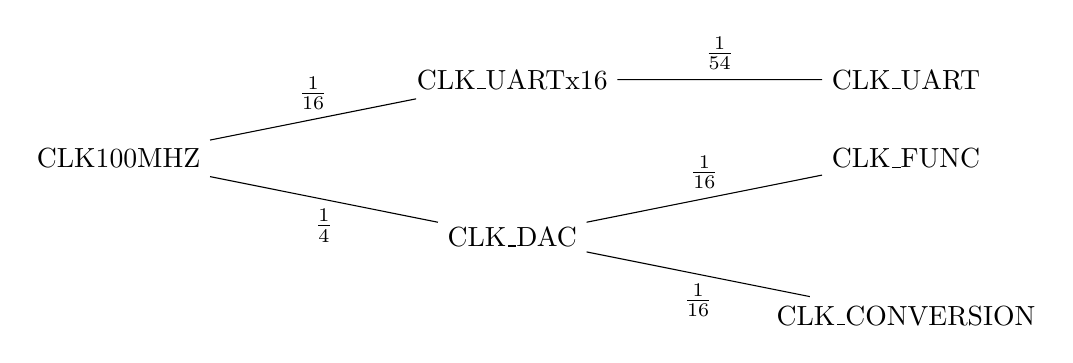
\begin{tikzpicture} 
    \node {CLK100MHZ}[grow=east, sibling distance=2cm, level distance=5cm]
    child {node {CLK\_DAC}
      child {node {CLK\_CONVERSION}
        edge from parent node [below] {$\frac{1}{16}$}}
      child {node {CLK\_FUNC}
        edge from parent node [above] {$\frac{1}{16}$}}
      edge from parent node [below] {$\frac{1}{4}$}}
    child {node {CLK\_UARTx16}
      child {node {CLK\_UART}
        edge from parent node [above] {$\frac{1}{54}$}}
      edge from parent node [above] {$\frac{1}{16}$}};
  \end{tikzpicture} 
  \caption{Clock-Tree des Funktionsgenerators. } \label{Comp:clk:clocktree}
\end{figure}


